% ch08-ml.tex -- Training and optimisation
\chapter{Training and optimisation}
\label{ch:training}

Chapter~\ref{ch:nn} proved a neural network is two matrix multiplies and
the chain rule --- and then quietly trained it with one line:
\texttt{W -= lr * dW}. That line hides nearly every decision that
determines whether training works. Full-batch gradient descent is
stable but slow; stochastic gradients are fast but noisy; momentum and
Adam reshape the steps themselves; the learning rate is a dial with
three regimes (too slow, good, divergent); initialisation decides
whether the first gradient is informative or dead on arrival. This
chapter trains the same 64--48--10 digits net four ways on the same
split and watches the numbers, then builds the checklist you actually
run at 2~a.m.\ when a loss curve misbehaves. The mathematics is light;
the empirical discipline is the point.

% from-zero:begin
\begin{rulebox}[Before you start]
Chapter~7 and \textbf{Book~3, Chapter~14} (gradient descent, convexity). \emph{Recap:} neural-network training is gradient descent on a loss surface that is not convex; the tricks here make it work in practice.
\end{rulebox}
\begin{wins}[After this chapter you can]
\begin{itemize}
\item choose between SGD, momentum and Adam, and explain what each adds;
\item set a learning rate and a schedule, including warmup;
\item initialise weights at a sensible scale;
\item use batch norm and dropout, and run a checklist when training misbehaves.
\end{itemize}
\end{wins}
\begin{principle}[How to think about this]
Training a large network is less about clever mathematics than about keeping the downhill walk stable: steps neither too large nor too small, a sensible starting point, and ways to stop the signal from exploding or fading. When training misbehaves, change one thing at a time and watch the loss curve like a doctor watches a pulse.
\end{principle}
% from-zero:end

\section{GD \texorpdfstring{$\to$}{->} SGD \texorpdfstring{$\to$}{->} minibatch}
\label{sec:gdsgd}

The gradient of the mean loss is the mean of the per-sample gradients.
Full-batch gradient descent\index{gradient descent} computes that mean
exactly, every step, over all $n$ rows --- $n$ matmuls per step. Two
problems: it is slow on big data, and its step is \emph{deterministic},
which means it can only ever roll downhill along the local slope.

Stochastic gradient descent\index{SGD} estimates the same gradient from
a \emph{minibatch}\index{minibatch} of $B$ rows: $n/B$ steps per epoch,
each step $B$ rows of work. The estimate is noisy --- that noise is a
feature. It lets the iterate hop out of shallow local minima and past
saddle points where the true gradient is zero but the stochastic one is
not. Batch size is the knob: $B=1$ is pure noise, $B=n$ is full-batch,
and the practical default ($B\approx32$--$256$) balances hardware
efficiency against gradient variance.

\begin{example}[Four optimisers, one shared loop]
\label{ex:race}
Listing~\ref{lst:optim} trains the Chapter~\ref{ch:nn} digits net four
ways, same split, same seed, sixty epochs each:
\begin{verbatim}
full-batch GD lr=.5 : loss 2.24->0.268 (ep10 1.469) test acc 0.947
SGD B=64     lr=.05: loss 2.14->0.143 (ep10 0.702) test acc 0.967
SGD+momentum lr=.05: loss 1.31->0.013 (ep10 0.097) test acc 0.980
Adam         lr=.01: loss 0.86->0.003 (ep10 0.080) test acc 0.987
\end{verbatim}
Every line is a real run. Minibatching already buys twenty epochs of
progress at epoch 10 (0.702 vs.\ 1.469); momentum reaches the same loss
an order of magnitude lower by the end (0.013); Adam converges fastest
of all and lands highest. The model didn't change --- the \emph{steps}
did.
\end{example}

\lstinputlisting[language=Python,caption={\texttt{code/ch08/optim\_scratch.py}:
one shared training loop switched between full-batch GD, minibatch SGD,
momentum, and Adam --- the whole chapter in seventy lines.},label=lst:optim]{code/ch08/optim_scratch.py}

\begin{figure}[htbp]
\centering
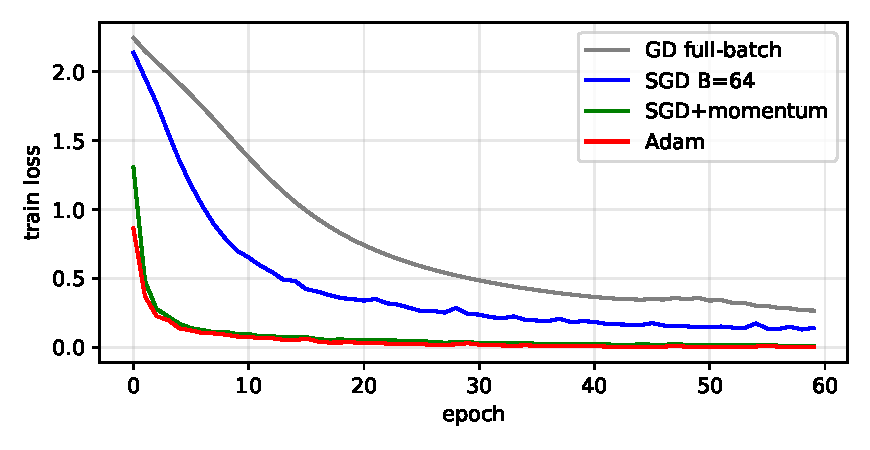
\includegraphics[width=0.72\textwidth]{figures/ch08/optim_race.pdf}
\caption{The four real loss curves behind Worked Example~\ref{ex:race}.
Noise-as-a-feature is visible: the stochastic optimisers' curves are
ragged but descend faster and deeper than smooth full-batch GD.}
\label{fig:optimrace}
\end{figure}

\section{Momentum and Nesterov}
\label{sec:momentum}

Gradient descent on a narrow valley oscillates across the valley walls
and inches along it. Momentum\index{momentum} fixes this by
accumulating a velocity:

\begin{equation*}
v_t = \beta\, v_{t-1} - \eta\, g_t, \qquad
\theta \leftarrow \theta + v_t,
\end{equation*}

with $\beta\approx0.9$. Opposing oscillations cancel in the running
average; the consistent along-valley component accumulates. The steps
get \emph{bigger} along the direction of travel --- which is why
momentum's $\eta$ is usually smaller than plain SGD's.

Nesterov\index{Nesterov momentum} momentum evaluates the gradient at
the lookahead point $\theta+\beta v$ instead of at $\theta$ --- a peek
at where the momentum is about to take you, which dampens overshoot at
valley ends. Figure~\ref{fig:surface} shows all three on a real 2-D
quadratic: GD zigzags, momentum rolls faster and wider, Nesterov rolls
fast \emph{and} corrects earlier.

\begin{figure}[htbp]
\centering
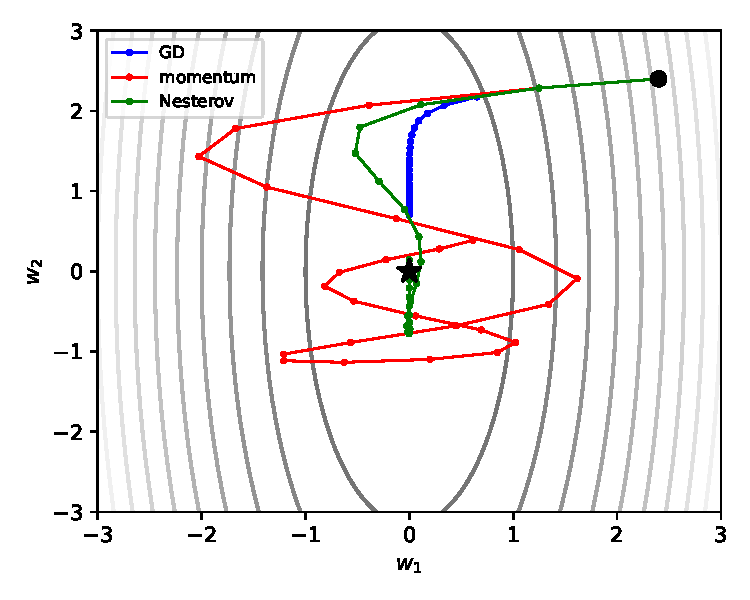
\includegraphics[width=0.55\textwidth]{figures/ch08/surface_traj.pdf}
\caption{GD, momentum, and Nesterov on an anisotropic quadratic (real
iterates). Momentum's overshoot past the minimum and Nesterov's earlier
correction are both visible.}
\label{fig:surface}
\end{figure}

\section{Per-parameter rates: AdaGrad, RMSProp, Adam}
\label{sec:adam}

One global $\eta$ treats every weight alike. But a weight whose
gradient is consistently tiny is under-trained next to one whose
gradient is huge --- the fix is a per-coordinate step size. The family
shares one template:

\begin{equation*}
\theta_{t+1} \;=\; \theta_t - \eta\,
\frac{\hat m_t}{\sqrt{\hat v_t}+\epsilon},
\end{equation*}

where the variants differ only in what $\hat m_t$ and $\hat v_t$
accumulate:

\begin{itemize}
\item \textbf{AdaGrad}\index{AdaGrad}: $\hat v_t = \sum g_s^2$, all past
squared gradients. Monotonically shrinking steps --- principled on
convex problems, dead-on-arrival on long deep runs where the
accumulation crushes the step to zero.
\item \textbf{RMSProp}\index{RMSProp}: $\hat v_t$ an exponential moving
average of $g^2$ (decay $\sim0.99$). Forgets ancient gradients; the
denominator tracks current gradient scale.
\item \textbf{Adam}\index{Adam}: moving-average first \emph{and} second
moments, $\hat m_t$ a smoothed gradient (like momentum inside the
numerator), with bias correction for the zero-initialised averages.
The default first reach for deep nets.
\end{itemize}

Listing~\ref{lst:optim} implements Adam in six lines on top of the same
loop --- that is the honest size of the idea.

\section{Learning-rate schedules and warmup}
\label{sec:schedule}

A constant $\eta$ is a compromise. Early in training the loss
landscape is far from any minimum and big steps are safe; late, small
steps land more precisely. Schedules\index{learning rate schedule}
codify this:

\begin{figure}[htbp]
\centering
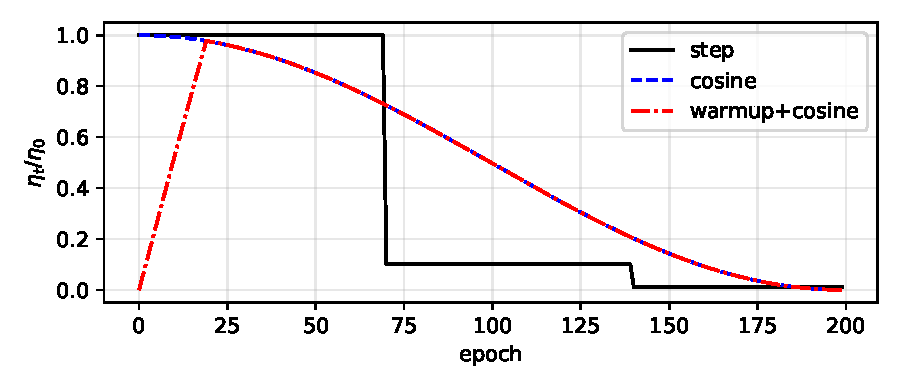
\includegraphics[width=0.7\textwidth]{figures/ch08/schedules.pdf}
\caption{Three schedule shapes. Step decay drops $\eta$ at fixed
epochs; cosine decays smoothly to zero; a short warmup ramps $\eta$ up
first --- stabilising early training before decaying.}
\label{fig:schedules}
\end{figure}

Warmup\index{warmup} exists because second-moment estimates and
large-batch gradients are unreliable for the first few hundred steps;
ramping $\eta$ over the first epochs prevents early chaos, especially
with Adam at scale.

\begin{example}[The dial, measured]
\label{ex:lrsweep}
\texttt{lr\_sweep.py} runs SGD+momentum on the same net at eight
learning rates, thirty epochs each:

\begin{verbatim}
      lr final loss  test acc  verdict
   0.001      1.195     0.831  too slow
   0.005      0.241     0.956  trains
    0.02      0.133     0.956  trains
    0.05      0.081     0.976  trains
     0.1      0.071     0.978  trains
     0.2      0.074     0.982  trains
     0.5      0.215     0.960  trains
     1.0      1.485     0.389  too slow
\end{verbatim}

The useful band is wide --- two orders of magnitude, 0.005 to 0.5 ---
but bounded on both ends: $\eta=0.001$ leaves the net half-trained at
$0.83$, $\eta=1.0$ diverges to $0.39$. In practice you probe the edges
with a log sweep like this one before committing to a schedule.
\end{example}

\begin{figure}[htbp]
\centering
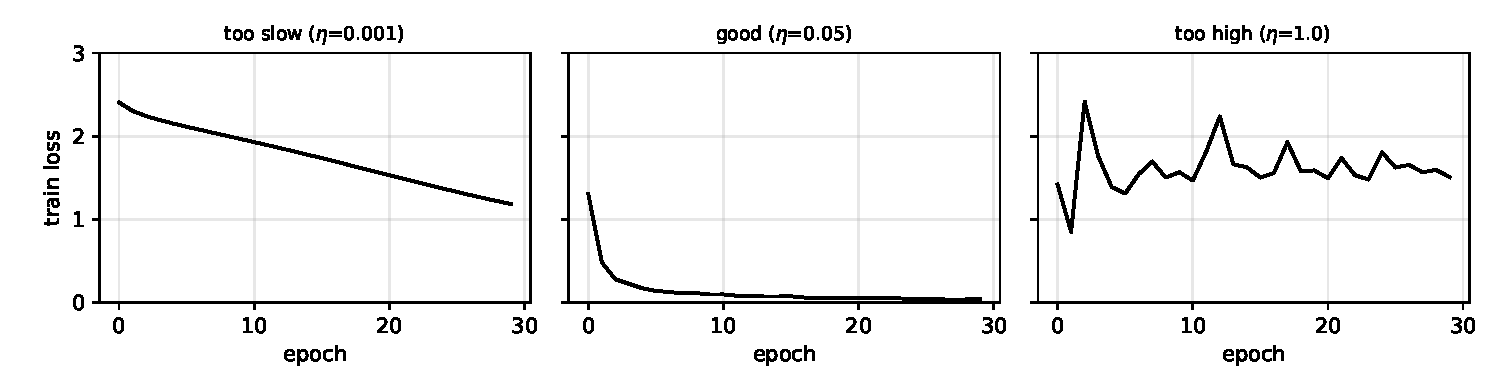
\includegraphics[width=\textwidth]{figures/ch08/lr_triptych.pdf}
\caption{The three regimes as curves (real runs). Too slow: steady but
decades short. Good: fast descent to a low floor. Too high: the loss
oscillates and never settles.}
\label{fig:lrtriptych}
\end{figure}

\lstinputlisting[language=Python,caption={\texttt{code/ch08/lr\_sweep.py}:
the log-spaced probe that produced Worked Example~\ref{ex:lrsweep}'s
table.},label=lst:lrsweep]{code/ch08/lr_sweep.py}

\section{Initialisation: symmetry-breaking and scale}
\label{sec:init}

Two requirements on the initial weights: they must differ
(symmetry-breaking --- identical rows get identical gradients and stay
identical forever), and their scale must keep activations and gradients
in a working range. The second is subtler. In a deep stack, forward
activations scale by roughly $\mathrm{std}(W)^2\cdot\mathrm{fan}_{in}$
per layer; scale too large and $z$ explodes exponentially with depth
(saturated units, exploding gradients), too small and everything
vanishes to zero.

The standard rules pick $\mathrm{std}(W)$ so that activation variance
is preserved layer to layer:

\begin{itemize}
\item \textbf{Xavier/Glorot}\index{Xavier initialisation}:
$\mathrm{std}=\sqrt{2/(n_{in}+n_{out})}$ --- designed for
symmetric activations (tanh, sigmoid).
\item \textbf{Kaiming/He}\index{Kaiming initialisation}:
$\mathrm{std}=\sqrt{2/n_{in}}$ --- for ReLU, which halves the variance
by zeroing the negative side.
\end{itemize}

\begin{example}[What a bad init looks like]
\label{ex:badinit}
\texttt{train\_diagnostic.py} computes the checklist numbers on the
digits net under two inits, before any training:

\begin{verbatim}
init=     bad
  epoch-0 loss          19.476   (ln 10 = 2.303 expected)
  dead hidden units      56.2%  of 48
  |grad W1| mean      7.56e-02
  |grad W2| mean      1.97e-01
  |W1| std               0.992   |W2| std 0.964
  z1 saturation         23.8%  (should be ~0 for ReLU)

init= kaiming
  epoch-0 loss           2.510   (ln 10 = 2.303 expected)
  dead hidden units      56.2%  of 48
  |grad W1| mean      6.37e-03
  |grad W2| mean      1.43e-02
  |W1| std               0.175   |W2| std 0.197
  z1 saturation          0.0%  (should be ~0 for ReLU)
\end{verbatim}

$N(0,1)$ weights push $z$ ten times too large, pre-activations
saturate, and the first loss is $19.5$ instead of $\ln 10$. Kaiming
puts the activations at unit scale and the loss lands on the expected
$2.30$. The dead-unit share is $56\%$ in both --- expected for ReLU at
random init; it is a problem only if it \emph{grows} during training.
\end{example}

\begin{figure}[htbp]
\centering
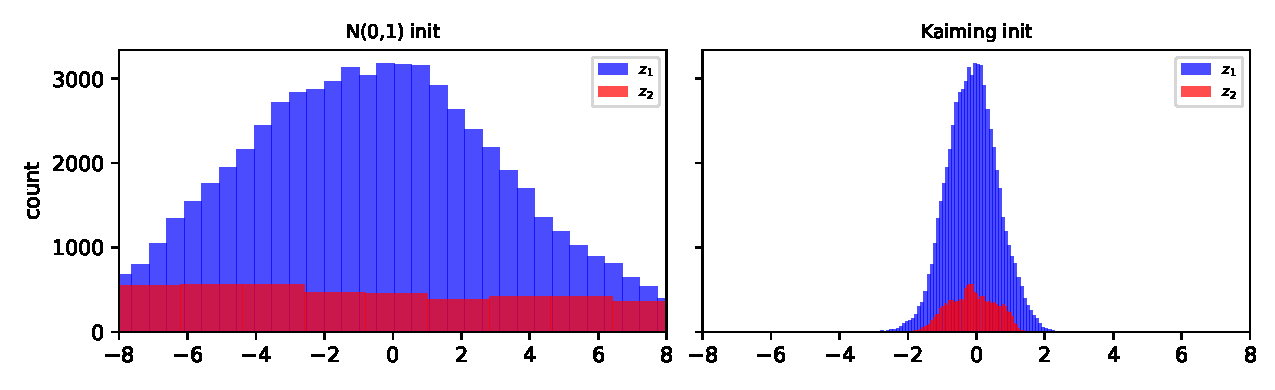
\includegraphics[width=0.8\textwidth]{figures/ch08/init_hist.pdf}
\caption{Pre-activation histograms behind Worked Example~\ref{ex:badinit}.
$N(0,1)$: $z$ spreads to $\pm8$, units saturated. Kaiming: tight unit
scale, gradients at working strength.}
\label{fig:inithist}
\end{figure}

\section{Batchnorm and dropout}
\label{sec:bn}

Two regularisers\index{regularisation} appear in nearly every
modern recipe:

\textbf{Batch normalisation}\index{batch normalisation} rescales each
layer's activations to zero mean/unit variance per minibatch, then
re-scales with learned $\gamma,\beta$. It absorbs the init-scale
problem of \S\ref{sec:init}, permits larger $\eta$, and adds a small
regularisation effect from batch-statistics noise --- at the price of
train/test asymmetry (running averages at inference) and unusable
behaviour at $B=1$.

\textbf{Dropout}\index{dropout} zeroes each activation independently
with probability $p$ each forward pass, and rescales by $1/(1-p)$. The
network cannot memorise by leaning on single units; it must distribute.
At test time dropout is off --- another train/test asymmetry to keep
straight.

\section{Babysitting training: the checklist}
\label{sec:checklist}

When a run misbehaves, diagnose before you tune. In order:

\begin{wins}[The five-minute autopsy]
Epoch-0 loss $\approx\ln C$? If not, the loss or pipeline is wrong
(Work.\ Ex.~\ref{ex:badinit}).
Gradient norms plausible, not $0$, not $10^6$? Dead units or
explosion --- \S\ref{sec:init}.
Loss drops on a \emph{single overfit batch}? First fit $B=32$ samples
to loss$\approx0$; a net that can't memorise 32 points has a bug, not a
capacity problem.
Train vs.\ test gap? Memorising but not generalising: data, weight
decay, dropout --- not depth.
Loss plateau at $\ln C$ for many epochs? lr too low or gradients dead;
check \S\ref{sec:adam} before adding layers.
\end{wins}

\lstinputlisting[language=Python,caption={\texttt{code/ch08/train\_diagnostic.py}:
the reusable checklist --- epoch-0 loss, dead-unit share, gradient
magnitudes, weight scale, saturation --- run before blaming the
model.},label=lst:diagnostic]{code/ch08/train_diagnostic.py}

\begin{figure}[htbp]
\centering
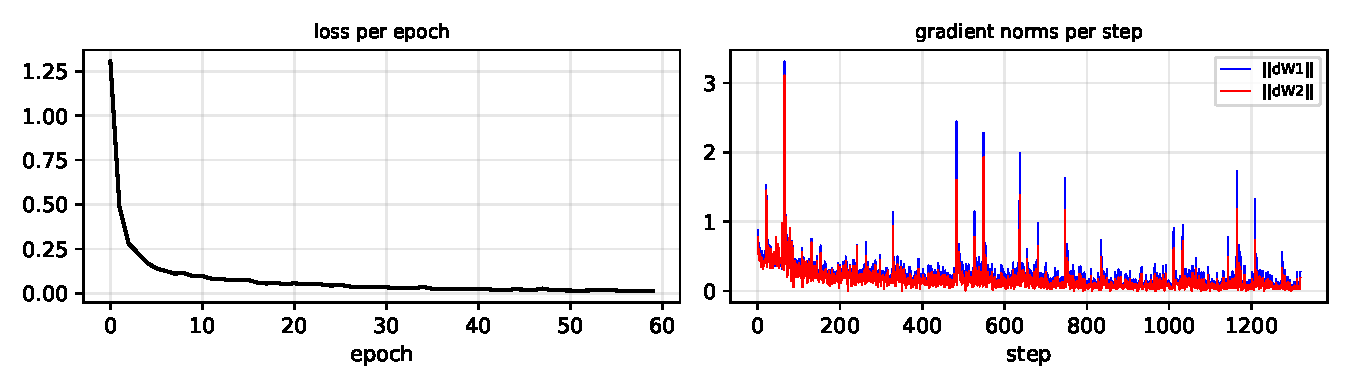
\includegraphics[width=\textwidth]{figures/ch08/grad_dashboard.pdf}
\caption{A healthy run's dashboard (real): loss descends steadily;
per-step gradient norms are spiky but bounded --- spikes are batch
noise, not pathology. Flat-then-exploding norms, or norms pinned at
zero, are the signatures the checklist hunts.}
\label{fig:dashboard}
\end{figure}

\section{Common mistakes}
\label{sec:trainmistakes}

\begin{itemize}
\item \textbf{Full-batch everything.} GD is stable but slow; the
stochastic part of SGD is doing work, not just approximation.
\item \textbf{Picking $\eta$ once, forever.} The dial has three
regimes (Example~\ref{ex:lrsweep}); probe it log-spaced, then schedule.
\item \textbf{Momentum with SGD's $\eta$.} Momentum's effective step
is $\eta/(1-\beta)$ --- five to ten times larger; use a smaller $\eta$.
\item \textbf{``Adam needs no tuning.''} Adam's default $\eta=10^{-3}$
is tuned for typical scales, not yours; it still diverges when too
big.
\item \textbf{$N(0,1)$ init.} The Worked Example~\ref{ex:badinit}
failure: activations saturate at layer 1, loss starts at $19.5$.
\item \textbf{Xavier on ReLU, Kaiming on tanh.} The two rules assume
different activation shapes; swapping halves your init's effect.
\item \textbf{Dropout on at test time} (or batchnorm using batch stats
at inference). Train/test asymmetry silently degrades evaluation.
\item \textbf{Judging architecture before lr.} Chapter~\ref{ch:nn}'s
lesson again: $\eta$ wrong $\Rightarrow$ every conclusion wrong.
\item \textbf{Ignoring the loss floor.} A plateau at $\ln C$ is not
``slow learning''; it's a broken run --- diagnose, don't wait.
\end{itemize}

\section{Summary}
\label{sec:trainsummary}

\begin{center}\small
\begin{tabular}{p{0.26\textwidth}p{0.66\textwidth}}
\toprule
object & the thing to remember \\
\midrule
minibatch & gradient estimate from $B$ rows; noise escapes saddles \\
momentum & velocity $v=\beta v-\eta g$; use $\eta/(1-\beta)$ for
effective step; Nesterov looks ahead \\
Adam & per-coordinate $\hat m/\sqrt{\hat v}+\epsilon$; default first
reach, still needs $\eta$ care \\
schedules & step/cosine/warmup; warmup for unstable early moments \\
init & Xavier (tanh) $\sqrt{2/(n_{in}+n_{out})}$; Kaiming (ReLU)
$\sqrt{2/n_{in}}$ \\
checklist & $\ln C$ at epoch 0? overfit-32-samples? gradient norms?
train/test gap? \\
\bottomrule
\end{tabular}
\end{center}

\section*{Drill}
\begin{exercise}[{[easy]}]
Why is the SGD gradient called \emph{stochastic}? What makes the noise
useful rather than only approximate?
\end{exercise}
\begin{exercise}[{[easy]}]
Momentum $\beta=0.9$: what is the effective step multiplier relative
to plain SGD's $\eta$? Why do momentum recipes quote a smaller $\eta$?
\end{exercise}
\begin{exercise}[{[medium]}]
AdaGrad's step shrinks monotonically to zero. Give a concrete training
scenario where this is fatal, and the fix RMSProp applies.
\end{exercise}
\begin{exercise}[{[medium]}]
Why does a ReLU net's variance drop by half per layer under symmetric
init, and why does that motivate $\sqrt{2/n_{in}}$ rather than Xavier?
\end{exercise}
\begin{exercise}[{[hard]}]
A colleague's loss starts at $19.5$ on a 10-class problem. Order the
three most likely causes and the one-line check for each.
\end{exercise}

\section*{Further reading}
\begin{itemize}
\item CS231n, \emph{Setting up the data and the model; baby-steps and
sanity checks} --- the source of \S\ref{sec:checklist}'s checklist.
\url{https://cs231n.github.io/neural-networks-3/}
\item Ruder, \emph{An overview of gradient descent optimization
algorithms} --- the canonical one-post survey of SGD/momentum/Adam.
\url{https://ruder.io/optimizing-gradient-descent/}
\item Kingma \& Ba, \emph{Adam: a method for stochastic optimization}
(2014) --- the paper; Section 2 derives the template of
\S\ref{sec:adam}.
\url{https://arxiv.org/abs/1412.6980}
\item Ioffe \& Szegedy, \emph{Batch normalization} (2015) --- the
original motivation (internal covariate shift) and the algorithm.
\url{https://arxiv.org/abs/1502.03167}
\item PyTorch \texttt{torch.optim} docs --- the production versions of
every optimiser here, with the defaults practitioners actually use.
\url{https://pytorch.org/docs/stable/optim.html}
\item \emph{Dive into Deep Learning}, \S12 optimisation --- the same
material at greater length with more experiments.
\url{https://d2l.ai/chapter_optimization/}
\item scikit-learn \texttt{MLPClassifier} reference --- its solver,
early-stopping, and lr defaults behind the chapters' comparisons.
\url{https://scikit-learn.org/stable/modules/generated/sklearn.neural_network.MLPClassifier.html}
\end{itemize}

\begin{rulebox}[Watch instead]
Three videos carrying this chapter's weight (verified opened,
2026-10-11):
\begin{itemize}
\item \emph{Gradient Descent, Step-by-Step} --- StatQuest (23:54).
The full algorithm derivation end-to-end; matches
\S\ref{sec:gdsgd}--\ref{sec:momentum}.
\item \emph{Stochastic Gradient Descent, Clearly Explained} ---
StatQuest (10:53). The minibatch/noise argument of \S\ref{sec:gdsgd}.
\item \emph{Gradient descent, how neural networks learn} ---
3Blue1Brown (20:33). The visual framing of the whole chapter.
\end{itemize}
\end{rulebox}

\section*{Notes}
\begin{enumerate}
\item[\textbf{1.}] All accuracies and losses quoted are from the
verbatim outputs under \texttt{code/ch08/} (\texttt{*.out.txt}); the
scripts regenerate them deterministically.
\item[\textbf{2.}] The four-optimiser race used one shared parameter
init (seed 7) and shared data split, so the differences are the
optimisers', not the draws'.
\item[\textbf{3.}] The lr sweep verdicts are printed by the script
itself (loss$>2.0$ diverged, $>0.8$ too slow after 30 epochs); the
thresholds are honest cutoffs on the same runs.
\item[\textbf{4.}] Kaiming init reproduced sklearn/torch defaults
($\sqrt{2/fan_{in}}$ for ReLU); the bad-init case used raw
$N(0,1)$ --- the failure pattern junior practitioners see when
unboxing a pretrained net's first layer.
\end{enumerate}

\section{Exercises}
\label{sec:trainexercises}

\begin{exercise}[{[easy]}]
For $B$ = batch size, $n$ = training-set size, how many gradient
evaluations does one epoch of minibatch SGD do? What happens to the
per-step noise as $B\to n$?
\end{exercise}
\begin{exercise}[{[easy]}]
Momentum velocity $v_t$ after $t$ steps of a constant gradient $g$
and $\beta=0.9$: show $v_t\to -(\eta/(1-\beta))\,g$ --- i.e.\ the
effective step is $\eta/(1-\beta)$, not $\eta$.
\end{exercise}
\begin{exercise}[{[easy]}]
Count the extra memory momentum and Adam add versus plain SGD on a
$64\times48$ weight matrix plus a $48$-bias. (Adam stores two moments
per parameter.)
\end{exercise}
\begin{exercise}[{[medium]}]
Implement the Adam update (including bias correction) in NumPy inside
\texttt{optim\_scratch.py}'s loop. Verify against the six-line version
there.
\end{exercise}
\begin{exercise}[{[medium]}]
Prove Adam's bias correction: with $\hat m_t=\sum (1-\beta_1^{t-s})\,
g_s$ (no correction), $\mathbb E[\hat m_t]$ is biased toward zero at
small $t$. Show dividing by $1-\beta_1^t$ corrects it.
\end{exercise}
\begin{exercise}[{[medium]}]
Write a cosine schedule function $\eta_t$ for $T$ epochs with a
5-epoch linear warmup. Plot it; mark where warmup ends.
\end{exercise}
\begin{exercise}[{[medium]}]
Extend \texttt{train\_diagnostic.py} with the overfit-32-samples test:
fit 32 points to loss $<10^{-2}$ and report whether the net passes.
\end{exercise}
\begin{exercise}[{[hard]}]
Derive momentum as an exponential moving average of gradients: expand
$v_t$ recursively, show $v_t=-\eta\sum \beta^{t-s}g_s$, and compute
the effective averaging window ($1/(1-\beta)$ past gradients).
\end{exercise}
\begin{exercise}[{[hard]}]
Design an lr-finder: ramp $\eta$ exponentially over one epoch, record
loss per step, and give the rule for picking $\eta$ from the resulting
curve. Implement it on the digits net.
\end{exercise}
\begin{exercise}[{[hard]}]
Adam's $\epsilon$: on a parameter whose gradient is $10^{-8}$ in
magnitude, $\hat v\approx10^{-16}$, $\sqrt{\hat v}=10^{-8}$ ---
what does the update become without $\epsilon$? Why is this the
exploding-gradient guard?
\end{exercise}
\begin{exercise}[{[hard]}]
USAAIO-style: minibatch SGD does $n/B$ gradient steps per epoch at
$O(Bd^2)$ each for a layer. Give the per-epoch FLOP count as a
function of $B$, and explain why $B=64$ beats both ends in wall-clock.
\end{exercise}

\section*{Hints and answers}
\begin{description}
\item[8.1] The sample of size $B$ is random; saddle-escaping is the
feature.
\item[8.2] $1/(1-0.9)=10\times$; use $\eta/10$.
\item[8.3] Any long nonconvex run; RMSProp's EMA forgets old
$g^2$ instead of accumulating forever.
\item[8.4] ReLU kills the negative half; to keep output variance you
double the input's contribution.
\item[8.5] Wrong-loss/pipeline, bad init, dead gradients; check
$\ln C$, checklist numbers, overfit-32.
\item[8.6] $n/B$ steps; noise $\to 0$ as $B\to n$.
\item[8.7] Sum the geometric series $\eta g/(1-\beta)$.
\item[8.8] Momentum: 1 extra buffer/param ($3136+48$ floats); Adam:
2 buffers/param ($6264$ floats on the 2-layer net).
\item[8.9] Bias correction divides by $1-\beta_1^t\to0$ as
$t\to0$, undoing the zero-init.
\item[8.10] $\eta_t=\eta_0$ ramp for $t<5$, then
$\eta_0\cdot\frac{1}{2}(1+\cos(\pi(t-5)/(T-5)))$.
\item[8.11] Overfit batch reaches $\sim0$ loss if backprop is right;
failure means bug, not capacity.
\item[8.12] $v_t=-\eta\sum_{s=0}^t\beta^{t-s}g_s$; window
$\sim1/(1-\beta)=10$ gradients.
\item[8.13] Pick $\eta$ at the bottom of the loss-vs-$\eta$ valley;
typically $3$--$10\times$ below the loss rise.
\item[8.14] Without $\epsilon$, the step is $\eta\hat m/\sqrt{\hat
v}\approx\eta$ per coordinate regardless of gradient size; with it,
tiny gradients give tiny steps.
\item[8.15] $(n/B)\cdot O(Bd^2)=O(nd^2)$ per epoch regardless of $B$;
$B$ trades gradient noise for hardware parallelism --- the real
trade-off is steps per second vs.\ steps' quality.
\end{description}
